\chapter{行波管的放大能力} \label{ch4}
行波管是一种放大微波信号的器件,因此放大能力是它的主要参数,并且通常用增益来表示。增益($ G $)的意义如下:
\begin{equation} \label{eq:ch4-1}
	G=10\lg\frac{P_\text{出}}{P_\text{入}}(\textrm{dB})
\end{equation}
其中$ P_\textrm{入} $为加到行波管输入端待放大信号的功率,而$ P_\text{出} $是在输出端得到的放大后的信号功率。$ G $的单位是分贝,$ G=10 $分贝相当于放大十倍;20分贝相当于放大100倍;30分贝相当于放大1000倍等等。

微波信号在行波管内所以能被放大,是因为在螺旋线内流动的电子注与外加信号所建立的高频场发生了能量转换的结果。因而行波管放大能力将主要由这两方面的条件及相互作用情况所决定。本章先着重定性讨论这些因素对行波管增益的影响,最后简略介绍一下增益计算的主要问题。
\section{电子注参量对增益的影响}
中小功率行波管中采用的电子注,基本上都是圆形截面的实心电子注。可以用三个参量来表征这种电子注的主要状况即:电子注电流$ I_0 $、电子速度$ v_e $(它是螺旋线电压$ U_0 $所决定)以及电子注截面半径$ b $。下面分别看看这三个因素改变时行波管增益如何随之变化。
\subsection{电子注电流的影响}	
	电子注电流($ I_0 $)越大,则参与同高频场相互作用的电子数目就相应增多。这就是说,有较多的电子受高频场的作用而群聚在减速场里,从而也就有更多的电子将其一部分动能转换为高频场的能量,使信号得到更充分的放大。所以电子注电流$ I_0 $增加对提高增益有利。
\subsection{电子注电压的影响}	
	电压$ U_0 $越高,则电子速度越快,惯性越大,因而在高频场作用下,就比较不容易改变其速度和位置,即不易很快地群聚起来。要使电子迅速群聚起来,就要有较强的高频电场,即需要在行波管输入端送进较强的信号功率($ P_\text{入} $)。否则,因电子注群聚较慢,输出端得到的放大后的信号功率就会减小。由\ref{eq:ch4-1}式可以看出,无论是输入功率$ P_\text{入} $增加,还是输出功率$ P_\text{出} $减小,都直接导致行波管的增益下降。所以,在同样的电子注功率(即:乘积$ U_0I_0 $)下,通常是较大的电流及较低的电压对提高管子增益有利些。	
	
	为了能够同时考虑电子注电流和电压增益的影响,常常使用一个叫“导流系数”的参量($ P_\theta $),它的定义是:
	\begin{equation} \label{eq:ch4-2}
		P_\theta = \frac{I_0}{U_0^{3/2}}
	\end{equation}
	
  由前面的讨论及导流系数的定义可以看出从提高行波管增益的角度考虑,希望电子注导流系数大些。但是,加大电子注导流系数,就要提高对磁聚束系统的要求,增加磁聚束的困难(见第\ref{ch7}章)。这就使电子注导流系数的提高受到一定限制。
	\subsection{电子注直径的影响}	
	我们由图\ref{ch3-6}已经知道,对于螺旋线慢波系统来说,螺旋线横截面内轴向电场的分布特点是:中心处最弱,沿半径方向由轴心往外逐渐增强,在接近导线表面时,轴向场达最大值。可见,如果螺旋线直径($ 2a $)及导波波长$ \lambda_g $一定,则随着电子注直径($ 2b $)的增大(即$ \frac{b}{a} $值增大),与电子注相互作用的平均轴向电场也相应增大,使电子注与高频场的相互作用增强。所以增大电子注直径对提高管子增益是有利的。但是应该指出随着电子注直径增大,电子注更加靠近螺旋线导丝,这就增加了电子被螺旋线截获的危险聚束性能就可能变坏。为了保证必要的聚束状态和聚束稳定性,通常$ \frac{b}{a} $值都在0.6以下。




\section{高频电场对增益的影响}
沿螺旋线传播一定功率的微波信号时,信号在电子注流经的地方所建立的高频电场的强弱及分布状况,直接影响着它与电子注能量交换的有效程度。从第三章关于螺旋线基本特性的介绍中我们知道,耦合阻抗Kc正是表征高频场与电子注相互作用有效程度的基本参量。耦合阻抗越高,则与电子注相互作用的高频电场越强,行波管的增益也就越高。


下面根据图\ref{ch3-8}所列曲线讨论一下影响螺旋线耦合阻抗$ K_c $(也就是影响与电子注相互作用的高频电场)的几个具体因素:
 \subsection{螺旋线直径对增益的影响}
	
	由图\ref{ch3-8}的曲线可以看出,当$ \gamma $及$ \frac{b}{a} $一定时,耦合阻抗$ K_c $





\begin{figure}[phtb]
	\centering
	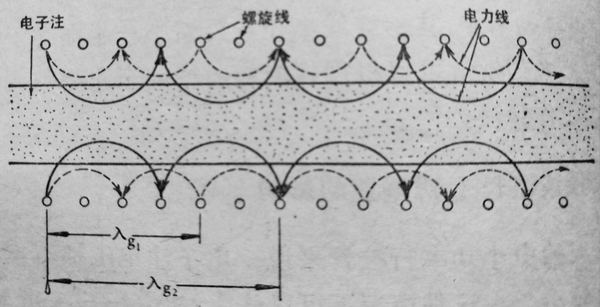
\includegraphics[width=0.65\linewidth]{figure/ch4-1}
	\caption{慢波波长改变时,高频场电力线形状变化示意图}
	\label{ch4-1}
\end{figure}

\begin{figure}[phtb]
	\centering
	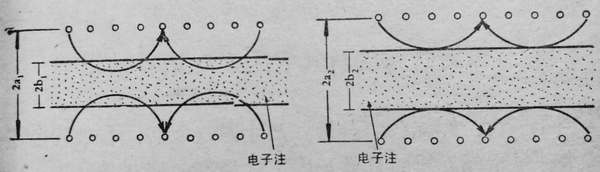
\includegraphics[width=0.65\linewidth]{figure/ch4-2}
	\caption{螺旋线直径增大后,进入电子注的电力线减少}
	\label{ch4-2}
\end{figure}

\begin{figure}[phtb]
	\centering
	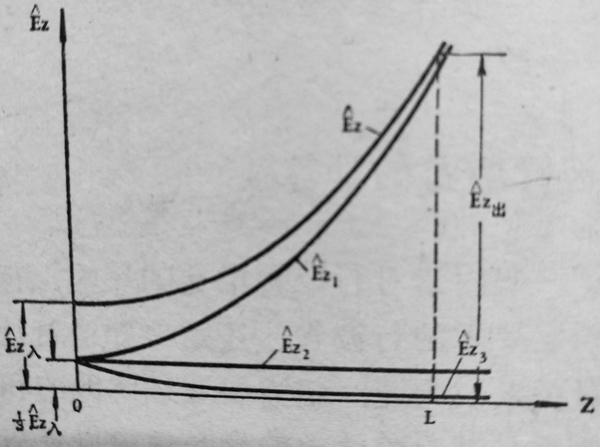
\includegraphics[width=0.65\linewidth]{figure/ch4-3}
	\caption{轴向高频电场沿$ Z $轴变化情况示意图}
	\label{ch4-3}
\end{figure}






